\subsection{Gestão de utilizadores}
Um requisito da aplicação e que apenas as empresas têm a possibilidade de se resgistarem, pelo que apenas estas poderão registar os seus técnicos. Para isso foi criada a página de gestão de utilizadores apenas acessível às empresas, nestas páginas estas poderão pesquisar pelos seus técnicos, ou registar novos técnicos, sendo que tem se ser obrigatóriamente indicado o nome, \textit{email} e tipo de utilizador. Outras ações que este utilizador poderá realizar é a visualizar um técnico onde poderá bloquear o acesso ou até apagar a conta do mesmo, sendo que esta ação e irreversível.


\begin{figure}[htb]%
  \centering
  \subfloat[\centering Aviso de impedir acesso à conta]{{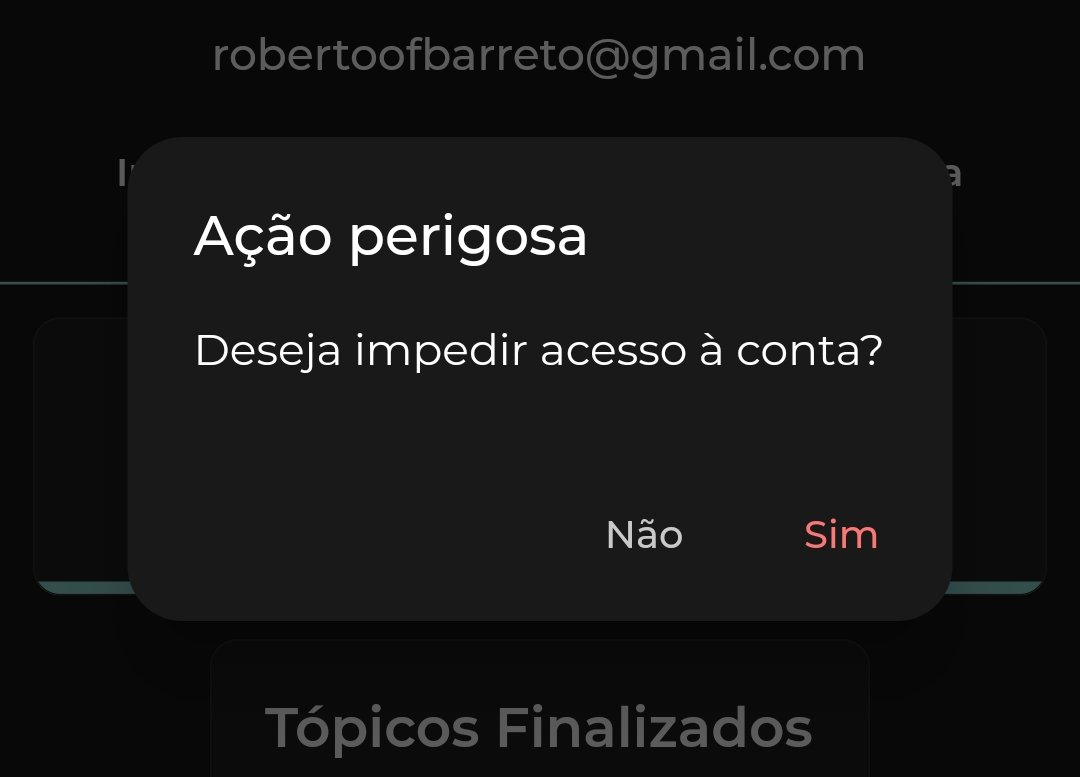
\includegraphics[width=0.4\textwidth]{images/implementacao/frontend/gestao_users/1686054310970.jpg} }}%
  \qquad
  \subfloat[\centering Aviso de remover conta]{{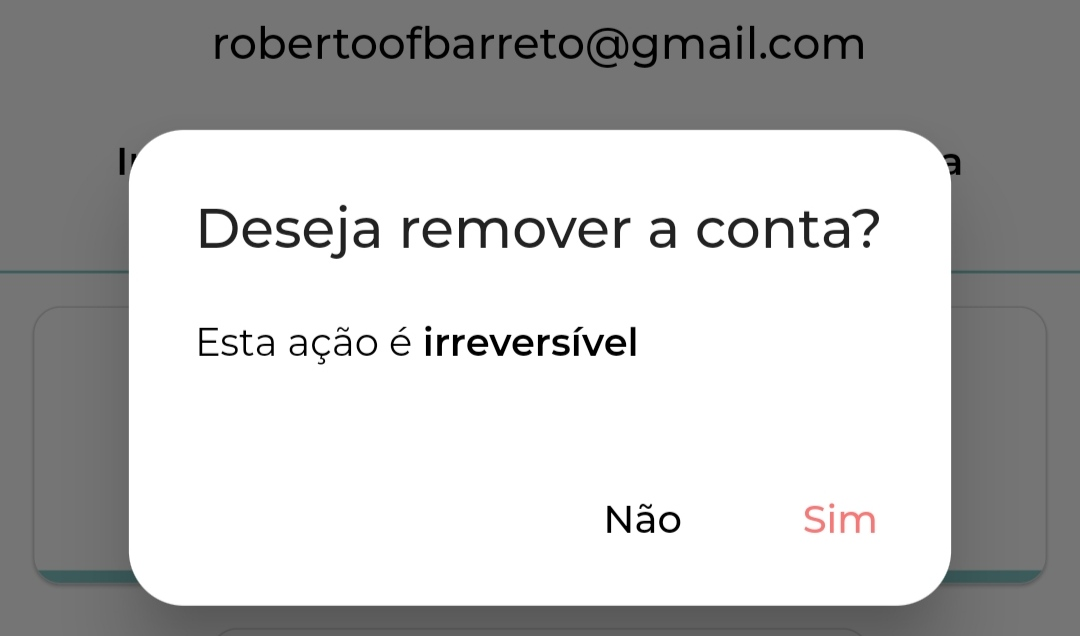
\includegraphics[width=0.4\textwidth]{images/implementacao/frontend/gestao_users/1686054218255.jpg} }}%
  \label{fig:70}%
\end{figure}

Sempre que um utilizador sem acesso ou com a conta apagada efetua o login, este receberá uma mensagem de erro mencionando que a sua este não possui acesso à conta impedindo assim o acesso.

\begin{figure}[htb]
  \centering
  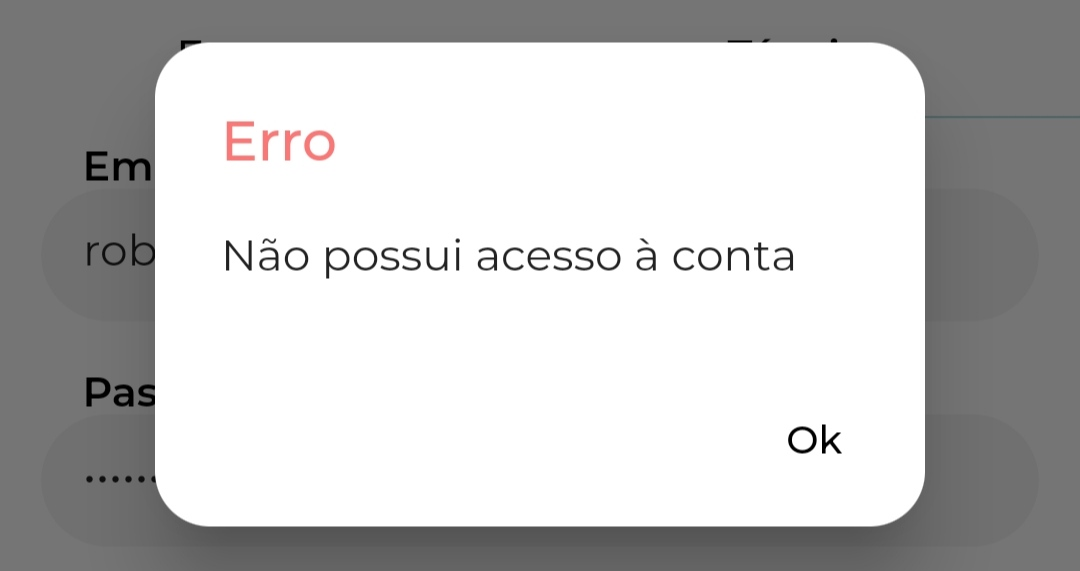
\includegraphics[width=0.4\textwidth]{images/implementacao/frontend/gestao_users/1686054218243.jpg}
  \caption{Aviso de login a conta sem acesso}
  \label{fig:71}
\end{figure}